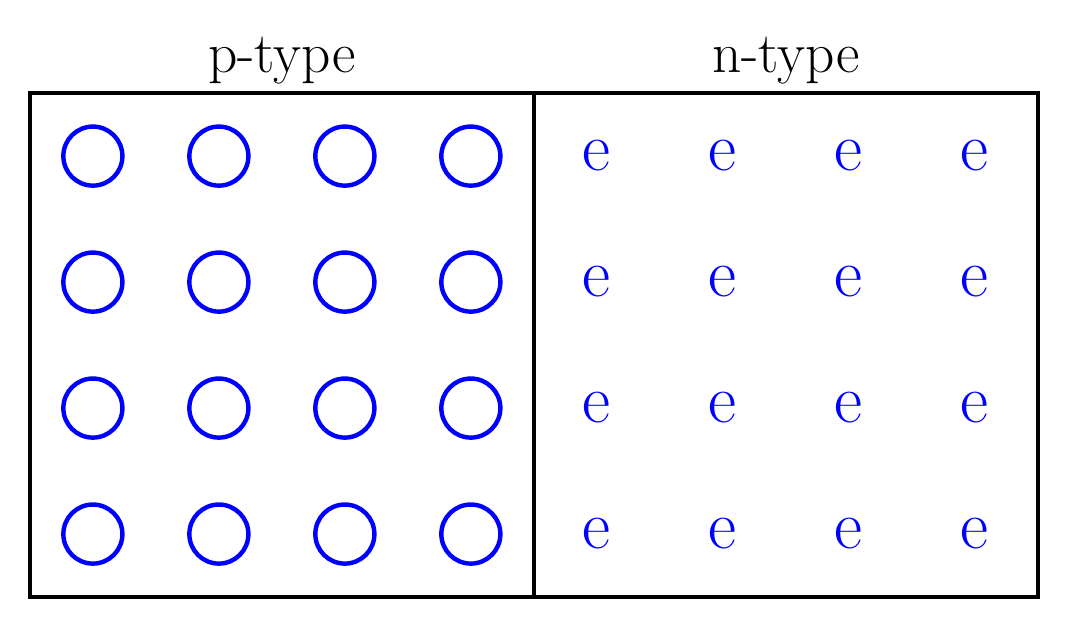
\begin{tikzpicture} [scale=0.8]                          
    \def\nx{8} % Number of dot x locations
    \def\ny{4} % Number of dot y locations
    \def\sep{2cm} % dot separation
    \def\re{0.75cm} % Electron size
    \def\c{blue} % Color of central nucleus and electrons
                                           
    % Semiconductor valence holes and conducting band electrons
    \foreach \ix in {0, ..., \inteval{\nx-1}}
        {
        \foreach \iy  in {0, ..., \inteval{\ny-1}}
            {
            \def\x{{(\ix+0.5)*\sep}}
            \def\y{{(\iy+0.5)*\sep}}
            \draw (\x,\y) coordinate(a);
            \pgfmathparse{less(\ix,\nx/2)}  
            \ifnum\pgfmathresult=1 % p-type
                \node at (a) [ultra thick, blue, circle, draw, minimum size = \re] {};
            \fi
            \pgfmathparse{greater(\ix,\nx/2-1)}  
            \ifnum\pgfmathresult=1 % n-type
                \node at (a) [blue] {\Huge e};
            \fi
            }
        }

    % Semiconductor boundaries and labels
    \draw[ultra thick] (0,0) rectangle ({\nx*\sep/2},{\ny*\sep});
    \node at ({\nx*\sep/4},{\ny*\sep}) [font=\huge, above] {p-type};
    \draw[ultra thick] ({\nx*\sep/2},0) rectangle ({\nx*\sep},{\ny*\sep});
    \node at ({3*\nx*\sep/4},{\ny*\sep}) [font=\huge, above] {n-type};        
      
\end{tikzpicture}